%%%%%%%%%%%%%%%%%%%%%%%%%%%%%%%%%%%%%%%%%%%%%%%%%%%%%%%%%%%%%%%%%%%%%%%%%%%%%%
%  Engineering Semantics for Trustworthy Industrial AI Agents:
%  A State-of-the-Art Survey and Capability Framework.
%  Every number, table and the PRISMA figure come from ../code/run_updated.py.
%%%%%%%%%%%%%%%%%%%%%%%%%%%%%%%%%%%%%%%%%%%%%%%%%%%%%%%%%%%%%%%%%%%%%%%%%%%%%%
\documentclass[10pt,journal,letterpaper]{IEEEtran}

\usepackage[T1]{fontenc}
\usepackage[utf8]{inputenc}
\usepackage{amsmath,amssymb}
\usepackage{booktabs}
\usepackage{array}
\usepackage{graphicx}
\usepackage{xcolor}
\usepackage{enumitem}
\usepackage{microtype}
\usepackage{tikz}
\usetikzlibrary{arrows.meta,positioning,fit,calc}
\usepackage{cite}
\usepackage{xurl}
\usepackage[hidelinks,breaklinks]{hyperref}

\makeatletter
\renewcommand{\paragraph}[1]{\par\vspace{2pt}\noindent\textbf{#1}\hskip 0.5em\ignorespaces}
\makeatother

\setlist{itemsep=0pt,topsep=2pt,parsep=0pt,partopsep=0pt}
\emergencystretch=2.5em
\newcolumntype{L}[1]{>{\raggedright\arraybackslash}p{#1}}
\setcounter{topnumber}{3}
\setcounter{dbltopnumber}{3}
\setcounter{totalnumber}{5}
\renewcommand{\topfraction}{0.92}
\renewcommand{\dbltopfraction}{0.92}
\renewcommand{\textfraction}{0.06}
\renewcommand{\floatpagefraction}{0.75}
\renewcommand{\dblfloatpagefraction}{0.75}

\newcommand{\opcua}{OPC~UA}
\newcommand{\AgentCatA}{0}
\newcommand{\AgentCatB}{0}
\newcommand{\AgentCatC}{0}
\newcommand{\AgentCatD}{0}
\newcommand{\AgentCatE}{0}
\newcommand{\AgentSystemsCoded}{0}
\newcommand{\AufAllThreeFirstClass}{0}
\newcommand{\AufAllThreeStrong}{1}
\newcommand{\AufAllThreeStrongNames}{MTP}
\newcommand{\AufAlpha}{pending}
\newcommand{\AufBehaviourFirstClass}{4}
\newcommand{\AufCells}{240}
\newcommand{\AufConstraintsFirstClass}{2}
\newcommand{\AufKappa}{pending}
\newcommand{\AufLocated}{0}
\newcommand{\AufProvenanceFirstClass}{5}
\newcommand{\AufTechnologies}{24}
\newcommand{\AufTypesFirstClass}{11}
\newcommand{\AufUncited}{1}
\newcommand{\AufUnitsFirstClass}{1}
\newcommand{\CsAasFacts}{411}
\newcommand{\CsAasPct}{57\%}
\newcommand{\CsAasTokens}{70,871}
\newcommand{\CsDisagreements}{0}
\newcommand{\CsFPRGFour}{0\%}
\newcommand{\CsFPRGOne}{0\%}
\newcommand{\CsFPRGThree}{0\%}
\newcommand{\CsFPRGTwo}{8\%}
\newcommand{\CsFPRGZero}{0\%}
\newcommand{\CsFacts}{726}
\newcommand{\CsKukaFacts}{676}
\newcommand{\CsKukaRetained}{676}
\newcommand{\CsOpcuaFacts}{507}
\newcommand{\CsOpcuaPct}{70\%}
\newcommand{\CsOpcuaTokens}{52,324}
\newcommand{\CsQkConflicts}{20}
\newcommand{\CsRecallGFour}{100\%}
\newcommand{\CsRecallGOne}{14\%}
\newcommand{\CsRecallGThree}{74\%}
\newcommand{\CsRecallGTwo}{68\%}
\newcommand{\CsRecallGZero}{0\%}
\newcommand{\CsSuffCFour}{86\%}
\newcommand{\CsSuffCOne}{0\%}
\newcommand{\CsSuffCThree}{51\%}
\newcommand{\CsSuffCTwo}{23\%}
\newcommand{\CsSuffCZero}{0\%}
\newcommand{\CsTopCFour}{100\%}
\newcommand{\CsTopCOne}{79\%}
\newcommand{\CsTopCThree}{100\%}
\newcommand{\CsTopCTwo}{95\%}
\newcommand{\CsTopCZero}{0\%}
\newcommand{\CsUnionFacts}{626}
\newcommand{\CsUnionPct}{86\%}
\newcommand{\RelatedSurveysVerified}{0}
\newcommand{\SurveyArxiv}{1186}
\newcommand{\SurveyAutoExcluded}{6373}
\newcommand{\SurveyCrossref}{9000}
\newcommand{\SurveyDuplicates}{3797}
\newcommand{\SurveyFailedSources}{none}
\newcommand{\SurveyFamilies}{9}
\newcommand{\SurveyHarvestDate}{2026-10-20}
\newcommand{\SurveyHarvestProtocolVersion}{1.1.0}
\newcommand{\SurveyIdentified}{17197}
\newcommand{\SurveyIncluded}{0}
\newcommand{\SurveyOpenAlex}{7011}
\newcommand{\SurveyPendingTA}{7027}
\newcommand{\SurveyProtocolVersion}{1.1.1}
\newcommand{\SurveyRelatedCandidates}{404}
\newcommand{\SurveyUnique}{7027}


\begin{document}

\title{Engineering Semantics for Trustworthy Industrial AI Agents: A State-of-the-Art Survey and Capability Framework}

\author{Anand~Todkar, Jitendra~Solanki, Mrinmoy~Sarkar%
\thanks{A. Todkar, J. Solanki, and M. Sarkar are with Siemens Foundational Technology, Siemens AG.
E-mail: anand.todkar@siemens.com; jitendra.solanki@siemens.com; mrinmoy.sarkar@siemens.com.}%
\thanks{Search protocol, screening and coding sheets, and the code that regenerates every number
in this paper are released with the article.}}

\maketitle

\begin{abstract}
Industrial AI agents increasingly read plant data and propose actions, yet language-model
reasoning alone does not establish which equipment is meant, in which unit a value is
expressed, whether a command is legal in the current state, whether a guard is satisfied,
or whether the evidence is current. Industrial information standards and semantic
technologies supply much of this knowledge, but surveys have treated industrial language
models, knowledge graphs, information models and semantic interoperability separately.
This survey analyses the field from the perspective of the engineering evidence an agent
needs. We define a reproducible review protocol with six research questions, five search
families and explicit inclusion, quality and coding rules, and we derive an
agent-usability framework (AUF) of ten capabilities, from identity to deployability, that
links engineering information to agent failure modes. Using AUF, we code
\AufTechnologies{} standards and vocabularies across five layers of the
engineering-semantics landscape and classify industrial agent architectures into five
grounding categories. Type and access semantics are widely standardised
(\AufTypesFirstClass{} technologies first class), whereas first-class unit
(\AufUnitsFirstClass{}), behaviour (\AufBehaviourFirstClass{}) and constraint
(\AufConstraintsFirstClass{}) semantics are rare, and \AufAllThreeFirstClass{} technologies
are first class in all three. A controlled case study illustrates the consequences: exposing these
capabilities raises declared-evidence sufficiency from \CsSuffCTwo{} to \CsSuffCFour{} and
fault recall from \CsRecallGTwo{} to \CsRecallGFour{}; equally informed procedural and SHACL
validators reach identical decisions; and matched OPC~UA and AAS projections of one
plant recover complementary facts, \CsOpcuaPct{} and \CsAasPct{} respectively, while
neither carries topology, legal commands, interlocks or observation time. We conclude
that agent reliability depends on a coherent runtime evidence contract rather than on a
particular syntax, and set out a research agenda for agent-ready industrial standards.
\end{abstract}

\begin{IEEEkeywords}
Industrial AI agents, large language models, engineering semantics, semantic
interoperability, OPC UA, Asset Administration Shell, knowledge graphs, runtime
validation, systematic review.
\end{IEEEkeywords}

\section{Introduction}
\label{sec:intro}

\PARstart{A}{request} such as ``raise the fill volume on Line~1 to 330\,mL'' carries obligations that a
fluent answer does not discharge. The agent must identify the filler and its writable
setpoint rather than a similarly described measurement, interpret the unit, obtain current
evidence, and respect the machine's operating state and process interlocks. These are
supervisory decisions above the controller's deterministic loop; an agent's plausible
response is not evidence that the proposed command is admissible.

Industrial automation has standardised much of the required knowledge over three decades:
\opcua{} information models \cite{iec62541}, the Asset Administration Shell (AAS)
\cite{idta2023aas}, property dictionaries \cite{eclass,iec61360}, ISA-95 hierarchies
\cite{iec62264}, PackML state machines \cite{isa88} and the Module Type Package
\cite{vdi2658}. The semantic web contributes RDF, OWL, SHACL and SPARQL
\cite{w3c2014rdf,w3c2012owl,knublauch2017shacl,w3c2013sparql}, together with QUDT units
\cite{qudt} and SOSA/SSN observations \cite{haller2019ssn}. These technologies were designed
for machine-to-machine interoperability. Whether they supply what a language agent needs at
decision time, and in which combination, has not been analysed systematically.

Existing reviews examine industrial language models, industrial knowledge graphs,
semantic interoperability and individual standards largely independently, and evaluate
technologies against interoperability criteria such as coverage, mapping effort and
conformance. Grounding research, conversely, evaluates retrieval and tool use on
open-domain data that has no units, interlocks or operational consequences
\cite{lewis2020rag,edge2024graphrag,pan2024unifying,patil2024gorilla}. The gap is an
analysis of the field from the perspective of the \emph{engineering evidence} an agent
requires to ground observations and actions.

The central question of this survey is therefore: \emph{what engineering information and
semantic capabilities are required to ground trustworthy industrial AI agents, how well do
existing industrial standards and semantic technologies provide them, and which gaps remain
for deployment?} We contribute:
\begin{enumerate}[label=\textbf{C\arabic*.},leftmargin=2.3em]
  \item A reproducible review protocol with six research questions, five search families,
  explicit eligibility, quality and coding rules, and released screening tooling
  (Section~\ref{sec:method}).
  \item The agent-usability framework (AUF): ten capabilities, each with a definition,
  the agent failure it prevents, a scoring rubric and supporting sources, used as the
  survey's coding instrument (Section~\ref{sec:auf}).
  \item A cross-technology capability analysis of \AufTechnologies{} standards and
  vocabularies organised in a five-layer engineering-semantics landscape
  (Sections~\ref{sec:landscape}--\ref{sec:capabilities}).
  \item A classification of industrial agent architectures by grounding source and
  authority, coded with AUF (Section~\ref{sec:agents}), and a reference synthesis
  derived from it (Section~\ref{sec:architecture}).
  \item A controlled case study showing how capability omissions identified by AUF manifest
  as grounding and validation failures, including a matched \opcua{}/AAS comparison
  (Section~\ref{sec:case}), and a research agenda (Section~\ref{sec:challenges}).
\end{enumerate}
The novelty lies in the analysis perspective, not in any individual technology: we
organise the field around the evidence contract that connects engineering information to
agent failure modes, and map it simultaneously across standards, semantic technologies and
agent architectures.

\section{Background and Related Surveys}
\label{sec:background}

\paragraph{Industrial agents.} We use \emph{industrial AI agent} for a system in which a
language model interprets an operator or system goal, retrieves plant information, and
produces answers or typed tool calls that may affect equipment. Tool use and reasoning
loops \cite{schick2023toolformer,yao2023react} and function-calling benchmarks
\cite{patil2024gorilla} established the general pattern; protocols such as MCP \cite{mcp}
standardise tool transport, not equipment truth.

\paragraph{Engineering semantics.} By \emph{engineering semantics} we mean
machine-interpretable statements about plant identity, types, units, structure,
behaviour, constraints and provenance, as carried by information models, property
dictionaries, ontologies and constraint languages. \emph{Grounding} is the resolution of an
utterance or proposal to such statements; \emph{validation} checks a proposal against
them before dispatch.

\paragraph{Knowledge-graph grounding.} Retrieval-augmented generation conditions output on
retrieved evidence \cite{lewis2020rag}; graph-based and hybrid variants retrieve structured
neighbourhoods \cite{edge2024graphrag,sarmah2024hybridrag}, and knowledge-graph/LLM
integration has been surveyed \cite{pan2024unifying}. These works mostly extract graphs from
text. Industrial evidence such as units, ranges, access rights, state machines and
interlocks is rarely written in text and must come from engineering systems. Our earlier
IIH Semantics framework \cite{todkar2025semanticitot} integrates \opcua{} aggregation,
RDF/SPARQL and a generated GraphQL schema on Industrial Edge; this survey generalises the
question beyond one architecture.

\paragraph{Related surveys.} Reviews of semantic interoperability evaluate standards for
machine-to-machine exchange, and reviews of LLMs in manufacturing evaluate applications or
models. Table~\ref{tab:related-surveys} positions this survey against reviews identified
by the protocol of Section~\ref{sec:method}; rows are added only after full-text
verification (\RelatedSurveysVerified{} verified at the time of writing). The
distinguishing combination is an agent-oriented capability framework applied jointly to
standards, semantic technologies and agent architectures with a systematic method.

\begin{table}[t]
\centering\footnotesize
\setlength{\tabcolsep}{3pt}
\caption{Scope of existing surveys versus this survey (\checkmark{} central, (\checkmark) partial). Agt.: industrial LLM agents; KG: industrial knowledge graphs; IM: information models; Int.: semantic interoperability; Val.: runtime validation; Fw.: capability framework; Sys.: systematic method. Rows are added only after the authors verify each survey's full text.}
\label{tab:related-surveys}
\begin{tabular}{@{}lccccccc@{}}
\toprule
Survey & Agt. & KG & IM & Int. & Val. & Fw. & Sys. \\
\midrule
\textbf{This survey} & \checkmark & \checkmark & \checkmark & \checkmark & \checkmark & \checkmark & \checkmark \\
\bottomrule
\end{tabular}
\end{table}


\section{Survey Methodology}
\label{sec:method}

\subsection{Research questions}
\begin{enumerate}[label=\textbf{RQ\arabic*.},leftmargin=2.6em]
  \item Which engineering-information capabilities do industrial AI agents require to
  ground observations and actions?
  \item Which standards, information models, semantic technologies and knowledge
  representations provide them?
  \item Where do current industrial-agent architectures obtain identity, units, topology,
  behaviour, constraints, provenance and runtime state?
  \item Which capabilities remain missing or weakly supported?
  \item Which architectural patterns combine LLM reasoning with deterministic engineering
  validation?
  \item What evidence shows that engineering semantics improve grounding, action
  correctness, transferability, auditability or context efficiency?
\end{enumerate}
RQ1 is answered by the AUF derivation (Section~\ref{sec:auf}), RQ2 by the technology
landscape and matrix (Sections~\ref{sec:landscape}--\ref{sec:capabilities}), RQ3--RQ5 by
the agent-literature coding (Sections~\ref{sec:agents}--\ref{sec:architecture}), and RQ6
by the reported evaluations and the case study (Section~\ref{sec:case}).

\subsection{Sources and search strategy}
Four evidence streams are distinguished and never pooled. \emph{Specifications} (IEC,
ISO, ISA, VDI/VDE/NAMUR, W3C, ETSI, OPC Foundation, IDTA, ECLASS, GS1, IDSA) are collected
from the issuing bodies and scored on what they standardise. \emph{Peer-reviewed
literature} published 2021--2026 is searched in IEEE Xplore, Scopus, Web of Science, ACM
Digital Library, ScienceDirect and SpringerLink by the authors, and in OpenAlex and
Crossref by released tooling; Crossref is relevance-ranked and capped, so it supplements
rather than replaces the boolean database searches. \emph{Preprints} (arXiv, posted
content) are coded but labelled non-peer-reviewed. \emph{Vendor material} supports only
implementation-capability statements. Foundational earlier work (retrieval augmentation,
tool use, constraint languages) enters through backward snowballing. Rather than one
query, the protocol defines eight topical families, (F1) LLM agents in industrial
automation and cyber-physical systems, (F2) industrial knowledge graphs and ontologies with
LLMs, (F3) \opcua{}, AAS and AutomationML with LLMs or agents, (F4) runtime validation and
guardrails in control systems, (F5) semantic grounding and interoperability, (F6) Graph- and
KG-RAG on engineering data, (F7) neurosymbolic, ontology-grounded and typed-tool agents, and
(F8) safety, provenance and trust, plus a family (R1) dedicated to related surveys. Exact
database-specific strings are frozen in protocol v\SurveyProtocolVersion{}, released with
the article; forward and backward snowballing from included studies complements them.

\subsection{Eligibility, screening and quality}
Studies are included if they address industrial AI or LLM agents or the engineering
semantics they consume (I1), industrial information models or knowledge graphs with an AI
consumer (I2), grounding, tool use, retrieval or runtime action validation in an
engineering context (I3), or constraints, provenance or state models used to check AI
outputs (I4). Exclusion codes are: no industrial context (E1); generic RAG or graph
construction without engineering semantics (E2); no agent or LLM (E3); duplicate or
superseded version (E4); insufficient documentation (E5); inaccessible full text (E6);
language or period (E7). Surveys (I5) feed only the related-survey gap analysis. Records are
deduplicated by DOI and by normalised title, year
and first author; near-identical titles are listed for manual resolution rather than
merged. A deterministic, versioned automation rule then marks records ineligible unless
title or abstract contains both an AI/semantics term and an industrial term; every
excluded record and the failing rule are released, as PRISMA~2020 requires for automation
tools. Title/abstract and full-text screening use spreadsheets that preserve each
decision and reason. A seeded random 20\% sample is designated for double coding at both
stages. Five quality items (architecture described, evaluation method, artefact
availability, isolation of the semantic contribution, safety limitations) are scored 0--2
and reported, not used for exclusion.

\subsection{Coding and agreement}
Each included system is coded for grounding category (Section~\ref{sec:agents}), retrieval
mechanism, tool interface, representation, each AUF capability on a 0--3 scale (absent,
implicit, explicit, checked at runtime), runtime validation, controller authority and
evaluation level (none, simulation, testbed, physical). Technologies are coded with the
rubric in Table~\ref{tab:rubric}, and each score is linked to a specification reference.
Agreement on the double-coded sample is reported as quadratic-weighted Cohen's $\kappa$
and ordinal Krippendorff's $\alpha$ with adjudicated disagreements; at the time of writing
the second rater's coding is pending ($\kappa$: \AufKappa{}, $\alpha$: \AufAlpha{}), and all
scores are first-rater codes.

\subsection{Capability levels}
Every capability statement records its level: \emph{specification} capability (what a
standard can express by default), \emph{implementation} capability (what a cited
implementation or profile exposes), and \emph{runtime} availability (what the agent
actually receives or checks when deciding). Matrix A (Section~\ref{sec:capabilities}) codes
specification capability; Matrix B (Section~\ref{sec:agents}) codes runtime availability
and records ``not reported'' rather than inferring capabilities a paper does not
demonstrate.

\subsection{Search status}
Figure~\ref{fig:prisma} is generated from the screening sheets. The open-source harvest
(\SurveyHarvestDate{}) identified \SurveyIdentified{} records (\SurveyCrossref{} Crossref,
\SurveyArxiv{} arXiv, \SurveyOpenAlex{} OpenAlex; incomplete for: \SurveyFailedSources{}).
After removing \SurveyDuplicates{} duplicates and marking \SurveyAutoExcluded{} records
ineligible by the automation rule, \SurveyUnique{} records await title/abstract
screening, and \SurveyRelatedCandidates{} industrial survey candidates await full-text
verification for Table~\ref{tab:related-surveys}. Subscription-database exports are
imported with the same tooling, after which all counts are regenerated.

\begin{figure}[t]
\centering
\resizebox{\linewidth}{!}{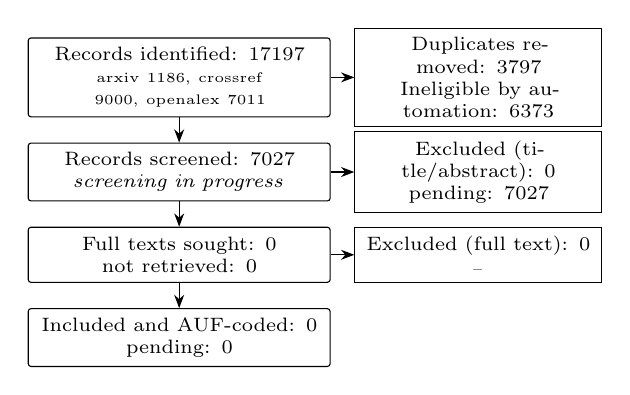
\begin{tikzpicture}[node distance=3.2mm and 3mm, >=Stealth]
\node[draw, rounded corners=1pt, align=center, font=\scriptsize, text width=3.6cm, minimum height=7mm] (id) {Records identified: 17197\\{\tiny arxiv 1186, crossref 9000, openalex 7011}};
\node[draw, align=center, font=\scriptsize, text width=2.9cm, minimum height=7mm, right=of id] (dup) {Duplicates removed: 3797\\Ineligible by automation: 6373};
\node[draw, rounded corners=1pt, align=center, font=\scriptsize, text width=3.6cm, minimum height=7mm, below=of id] (scr) {Records screened: 7027\\\textit{screening in progress}};
\node[draw, align=center, font=\scriptsize, text width=2.9cm, minimum height=7mm, right=of scr] (tax) {Excluded (title/abstract): 0\\pending: 7027};
\node[draw, rounded corners=1pt, align=center, font=\scriptsize, text width=3.6cm, minimum height=7mm, below=of scr] (ft) {Full texts sought: 0\\not retrieved: 0};
\node[draw, align=center, font=\scriptsize, text width=2.9cm, minimum height=7mm, right=of ft] (ftx) {Excluded (full text): 0\\{\tiny --}};
\node[draw, rounded corners=1pt, align=center, font=\scriptsize, text width=3.6cm, minimum height=7mm, below=of ft] (inc) {Included and AUF-coded: 0\\pending: 0};
\draw[->] (id) -- (scr); \draw[->] (scr) -- (ft); \draw[->] (ft) -- (inc);
\draw[->] (id) -- (dup); \draw[->] (scr) -- (tax); \draw[->] (ft) -- (ftx);
\end{tikzpicture}
}
\caption{PRISMA 2020 flow generated from the screening sheets; counts update automatically
as screening proceeds.}
\label{fig:prisma}
\end{figure}

\section{The Agent-Usability Framework}
\label{sec:auf}

An industrial agent receives a goal, resolves it against a plant it has not seen, decides
which evidence it needs, and proposes an answer or action that must be checkable before
dispatch. AUF asks what each source of engineering semantics contributes to that cycle.
The ten capabilities were derived by tracing the minimum evidence obligations of a
bounded supervisory cycle (resolve, interpret, locate, decide, check, trust, retrieve)
and the two cross-cutting feasibility conditions of a deployment (context budget and
ecosystem). Table~\ref{tab:rubric} states for each capability the operational requirement,
the agent failure it prevents, the scoring anchors and representative sources. The
derivation is tested against the coded literature as a saturation check: any recurring
requirement that cannot be mapped to U1--U10 is reported as a framework gap.

\begin{table*}[t]
\centering\footnotesize
\setlength{\tabcolsep}{3pt}
\caption{AUF capabilities: requirement, failure mode prevented and rubric anchors (0 absent;
1 incidental; 2 supported; 3 first class). Scores reflect what a specification
standardises by default, not optional extensions.}
\label{tab:rubric}
\begin{tabular}{@{}L{1.9cm}L{3.2cm}L{3.0cm}L{2.6cm}L{4.4cm}L{1.6cm}@{}}
\toprule
Capability & Requirement & Failure prevented & 1 incidental & 3 first class & Sources \\
\midrule
U1 Identity & resolve phrase to the right concept and instance & wrong equipment; homograph conflation & identifiers unique per vendor or file & globally unique, versioned, resolvable, synonym handling & \cite{iso29002,eclass,iec61360} \\
U2 Types and access & know datatypes, ranges, access rights & malformed call; write to read-only point & datatype only & datatypes, ranges, access rights, enumerations, run-time introspection & \cite{iec62541,patil2024gorilla} \\
U3 Quantities & bind values to quantity kind and unit & dimension or scale error & unit as display string & quantity kind, dimension vector, affine conversion & \cite{qudt} \\
U4 Relations & containment, topology, typed relations & wrong scope; missed impact & containment only & typed relations with transitivity and inverses & \cite{iec62264,balaji2016brick} \\
U5 Behaviour & operations, state machines, legal commands & command illegal in current state & operations named, untyped & typed operations plus state model with legality conditions & \cite{isa88,vdi2658} \\
U6 Constraints & checkable guards and envelopes & unsafe or out-of-envelope proposal & range or type checks & executable constraint language with reports & \cite{knublauch2017shacl,w3c2018odrl} \\
U7 Provenance and time & timestamped, attributed evidence & stale or untraceable evidence & one global timestamp & per-value time, source, agent and derivation & \cite{w3c2013prov,haller2019ssn} \\
U8 Query pushdown & filter, join, aggregate outside the model & context stuffing; unanswerable aggregates & filtered fetch & query language with joins, aggregation, path traversal & \cite{w3c2013sparql,edge2024graphrag} \\
U9 Context economy & faithful minimal evidence slice & budget exhaustion before evidence & verbose, partial fetch & compact and projectable to a minimal faithful slice & \cite{lewis2020rag,sarmah2024hybridrag} \\
U10 Ecosystem & implementations, converters, governance & deployment never happens & one implementation & open implementations, converters, reference data, active governance & \cite{idta2023aas,mcp} \\
\bottomrule
\end{tabular}
\end{table*}

Three design rules make AUF a repeatable instrument rather than an opinion table. First,
capabilities are scored separately, because strength in one does not compensate for
another: a \texttt{Double} in bar and a \texttt{Double} in psi have the same type, and a
complete address space need not state the order in which commands are legal. Second,
technologies are scored on their default specification, since that is what an agent
receives unless a deployment publishes more; deployment profiles are scored separately
when agent systems are coded. Third, U1--U8 are evidence obligations whereas U9--U10 are
feasibility conditions; AUF does not cover model training, cybersecurity or human
factors, and it does not prescribe a serialisation.

\section{Engineering-Semantics Technology Landscape}
\label{sec:landscape}

AUF states what an agent needs; the five layers state where capabilities come from. The
layers classify sources by role and are not an industrial reference architecture or a
strict dependency hierarchy: one standard may contribute to several layers, and a
deployment can combine them without materialising one graph. RAMI~4.0 remains the
reference architecture; the layers are a complementary evidence view.

\paragraph{L0: Identification and dictionaries.} ECLASS, IEC common data dictionaries and
IRDIs give properties stable, cross-vendor definitions \cite{eclass,iec61360,iec61987,iso29002};
GS1 identifiers distinguish products and individual assets. Concept identity is not
instance identity: identifying ``pressure'' does not identify the transmitter on one filler,
which needs asset membership and an observation source. Persistent identifiers also need
governed mappings when hardware is replaced.

\paragraph{L1: Information and interface models.} \opcua{} combines typed address spaces,
access levels, engineering ranges and callable methods, with companion specifications for
domain content \cite{iec62541}; the AAS supplies submodels with semantic identifiers
\cite{idta2023aas,idta2023nameplate}. AutomationML carries engineering exchange
\cite{iec62714}, ISA-95 equipment hierarchies \cite{iec62264}, and MTP and PackML services
and state machines \cite{vdi2658,isa88}; WoT Thing Descriptions, NGSI-LD and IEC~61850
provide further interface and entity models \cite{w3c2023wot,etsi2023ngsild,iec61850}. These
models make introspection and tool synthesis possible, but what a deployment exposes must
be audited: an agent cannot check an interlock that was never published, even when the
host standard could express it.

\paragraph{L2: Formal semantics, query and validation.} RDF provides globally named
relations, OWL entailment over classes and properties, SHACL closed-world checks of a data
graph against shapes, and SPARQL joins, traversal and aggregation outside the model
\cite{w3c2014rdf,w3c2012owl,knublauch2017shacl,w3c2013sparql}; PROV-O records derivation
and responsibility \cite{w3c2013prov}. Open-world consistency does not enforce mandatory
action parameters, and shape conformance does not establish that the engineering mapping
or the set of interlocks is complete.

\paragraph{L3: Quantities, observations and domain relations.} QUDT supplies quantity
kinds, dimension vectors and conversion factors \cite{qudt}; a display symbol such as
``bar'' does not itself state a conversion. SOSA/SSN separates sensors, observed properties,
observations and results \cite{haller2019ssn}, so that an answer can cite the measurement
and time it reports. Brick, SAREF and DEXPI contribute typed equipment and process
relations \cite{balaji2016brick,etsi2020saref,dexpi}; flow topology supports impact
analysis but not causal diagnosis without incident evidence.

\paragraph{L4: Cross-organisational policy and trust.} Dataspaces add participant identity,
catalogues, contracts and usage policies \cite{idsa2022ram,catenax}; ODRL expresses
permissions and duties \cite{w3c2018odrl}. Policy is a gate separate from physical
operating constraints, and an ODRL statement does not by itself enforce downstream use.

\section{Comparative Capability Analysis}
\label{sec:capabilities}

\begin{table*}[t]
\centering\footnotesize
\setlength{\tabcolsep}{3.4pt}
\caption{AUF coding of 24 standards and vocabularies (scores 0--3, rubric in Table~\ref{tab:rubric}). Scores describe what the specification standardises by default, not deployed profiles; single-rater (R1) coding, inter-rater agreement pending. $^\dagger$specification reference to be added.}
\label{tab:auf-matrix}
\begin{tabular}{@{}llcccccccccc@{}}
\toprule
L & Technology & U1 & U2 & U3 & U4 & U5 & U6 & U7 & U8 & U9 & U10 \\
\midrule
L0 & ECLASS / IEC CDD / IEC 61987 \cite{eclass,iec61360,iec61987,iso29002} & 3 & 2 & 2 & 1 & 0 & 1 & 0 & 1 & 2 & 3 \\
 & GS1 identifiers / EPCIS $^\dagger$ & 3 & 1 & 0 & 1 & 1 & 0 & 2 & 1 & 2 & 3 \\
\midrule
L1 & OPC UA core and companions \cite{iec62541} & 3 & 3 & 2 & 2 & 3 & 1 & 2 & 1 & 1 & 3 \\
 & Asset Administration Shell \cite{idta2023aas,idta2023nameplate} & 3 & 3 & 2 & 2 & 2 & 1 & 2 & 1 & 1 & 3 \\
 & AutomationML \cite{iec62714} & 2 & 3 & 1 & 3 & 1 & 1 & 1 & 0 & 1 & 2 \\
 & MTP \cite{vdi2658} & 2 & 3 & 2 & 2 & 3 & 2 & 1 & 0 & 2 & 2 \\
 & PackML \cite{isa88} & 1 & 2 & 0 & 0 & 3 & 2 & 0 & 0 & 3 & 3 \\
 & ISA-95 / IEC 62264 \cite{iec62264} & 2 & 2 & 1 & 3 & 1 & 0 & 1 & 0 & 2 & 3 \\
 & W3C WoT TD 1.1 \cite{w3c2023wot} & 3 & 3 & 2 & 1 & 3 & 1 & 1 & 1 & 2 & 2 \\
 & NGSI-LD \cite{etsi2023ngsild} & 3 & 2 & 2 & 3 & 1 & 1 & 3 & 2 & 2 & 2 \\
 & IEC 61850 \cite{iec61850} & 3 & 3 & 2 & 2 & 2 & 1 & 2 & 0 & 1 & 3 \\
\midrule
L2 & RDF / RDFS \cite{w3c2014rdf} & 3 & 2 & 0 & 3 & 0 & 0 & 1 & 3 & 1 & 3 \\
 & OWL 2 \cite{w3c2012owl} & 3 & 3 & 0 & 3 & 0 & 2 & 0 & 2 & 1 & 3 \\
 & SHACL \cite{knublauch2017shacl} & 2 & 3 & 1 & 2 & 1 & 3 & 1 & 2 & 2 & 3 \\
 & SPARQL 1.1 \cite{w3c2013sparql} & 2 & 1 & 0 & 3 & 0 & 1 & 1 & 3 & 3 & 3 \\
 & PROV-O \cite{w3c2013prov} & 3 & 2 & 0 & 3 & 1 & 0 & 3 & 2 & 2 & 2 \\
\midrule
L3 & QUDT \cite{qudt} & 3 & 2 & 3 & 1 & 0 & 2 & 0 & 2 & 2 & 2 \\
 & SOSA / SSN \cite{haller2019ssn} & 3 & 2 & 1 & 2 & 1 & 0 & 3 & 2 & 2 & 3 \\
 & Brick \cite{balaji2016brick} & 3 & 3 & 1 & 3 & 0 & 1 & 0 & 3 & 2 & 3 \\
 & SAREF and extensions \cite{etsi2020saref} & 3 & 2 & 2 & 2 & 2 & 0 & 1 & 2 & 2 & 2 \\
 & DEXPI \cite{dexpi} & 2 & 3 & 2 & 3 & 0 & 1 & 1 & 1 & 1 & 2 \\
\midrule
L4 & IDS-RAM / Dataspace Protocol \cite{idsa2022ram} & 3 & 2 & 0 & 2 & 1 & 2 & 3 & 1 & 1 & 2 \\
 & Catena-X / Manufacturing-X \cite{catenax} & 3 & 3 & 1 & 2 & 1 & 2 & 3 & 1 & 1 & 2 \\
 & ODRL \cite{w3c2018odrl} & 2 & 2 & 0 & 2 & 2 & 3 & 2 & 1 & 2 & 2 \\
\bottomrule
\end{tabular}
\end{table*}


Table~\ref{tab:auf-matrix} codes \AufTechnologies{} technologies (\AufCells{} cells).
Each row is linked to its specification; clause-level locators are being added to the
released evidence register (\AufLocated{} of \AufCells{} cells located,
\AufUncited{} row awaiting a specification reference). Reading the matrix by column
yields four observations.

\paragraph{Typing is solved; consequential semantics are sparse.} \AufTypesFirstClass{}
technologies are first class on U2, which explains why ``AI-ready'' data layers that expose
types appear convincing. First-class support is rare for units (\AufUnitsFirstClass{}),
behaviour (\AufBehaviourFirstClass{}) and constraints (\AufConstraintsFirstClass{}), the
capabilities that separate a well-typed proposal from an admissible one.

\paragraph{No single technology provides the evidence contract.} \AufAllThreeFirstClass{}
technologies are first class on all of U3, U5 and U6, and only \AufAllThreeStrong{}
(\AufAllThreeStrongNames{}) reaches at least ``supported'' on all three. An agent that
needs unit, behaviour and constraint evidence must therefore compose standards, for
example an information model for types and states, a unit ontology for conversion and a
constraint language for guards.

\paragraph{Richness and economy trade off.} The richest information models score lowest on
context economy (U9). This is not a defect of the standards but indicates that semantic
models belong behind query and projection interfaces rather than in prompts (U8).

\paragraph{Provenance is available but separate.} First-class provenance
(\AufProvenanceFirstClass{} technologies) concentrates in observation, provenance,
context-entity and dataspace models, whereas the machine-interface models \opcua{} and AAS
are only supported on U7. Freshness checks therefore require joining layers at runtime.

These observations concern what specifications standardise. Deployed profiles can expose
more (\opcua{} methods with state machines) or less (an AAS without constraint submodels),
which is why agent systems are coded on what they actually use
(Section~\ref{sec:agents}) and why the case study compares emitted profiles
(Section~\ref{sec:case}).

\section{State of the Art in Industrial Agent Grounding}
\label{sec:agents}

Published industrial agents differ less in the language model they use than in where their
engineering evidence comes from and who holds authority over actions. We therefore classify
systems into five grounding categories (Fig.~\ref{fig:categories}) and code each included
system with AUF on what it actually uses at runtime (Table~\ref{tab:agent-systems}).

\begin{figure}[t]
\centering\footnotesize
\setlength{\tabcolsep}{2pt}
\begin{tabular}{@{}cl@{}}
\toprule
& Pipeline \\
\midrule
A & LLM $\rightarrow$ documents, manuals $\rightarrow$ recommendation \\
B & LLM $\rightarrow$ typed tools $\rightarrow$ industrial API \\
C & LLM $\rightarrow$ knowledge-graph retrieval $\rightarrow$ engineering context \\
D & LLM $\rightarrow$ proposal $\rightarrow$ engineering validation $\rightarrow$ execution \\
E & LLM $\rightarrow$ validation $\rightarrow$ dispatch gate $\rightarrow$ controller checks $\rightarrow$ process \\
\bottomrule
\end{tabular}
\caption{Grounding categories used to code industrial agent systems. Categories are cumulative
in authority, not in capability: a C system may lack typed tools.}
\label{fig:categories}
\end{figure}

\paragraph{A: Document-grounded.} Retrieval over manuals, procedures and logs
\cite{lewis2020rag} grounds explanations and troubleshooting. Identity (U1) and units (U3)
remain implicit in text, so answers can be fluent yet unverifiable, and actions have no
checkable target.

\paragraph{B: Typed-tool grounded.} The model calls declared functions on \opcua{}, AAS or
vendor APIs \cite{schick2023toolformer,yao2023react,patil2024gorilla,mcp}. Schemas provide
types and access (U2) and can constrain identifiers, but units, state legality and guards
are only as explicit as the exposed interface; tool transport does not establish equipment
truth.

\paragraph{C: Knowledge-graph grounded.} Retrieval over engineering graphs supplies identity,
relations and query pushdown (U1, U4, U8) \cite{edge2024graphrag,sarmah2024hybridrag,pan2024unifying,todkar2025semanticitot}.
Graphs built from engineering systems carry facts that text-derived graphs cannot, but
retrieval quality and the completeness of the mapped constraints become new dependencies.

\paragraph{D: Semantically validated.} Proposals are lifted into a checkable form and
validated against constraints and state models (U5, U6) before execution
\cite{knublauch2017shacl}. Validation converts a claim into a proposition with a truth
value, but only relative to the constraints that were modelled.

\paragraph{E: Controller-authoritative.} Validation is repeated at dispatch with fresh
evidence (U7), and the controller retains independent, current-state checks and final
actuator authority. This category separates supervisory reasoning from deterministic
control and is the only one compatible with functional-safety practice; it is also the
least reported with physical evaluation.

\begin{table*}[t]
\centering\footnotesize
\setlength{\tabcolsep}{3pt}
\caption{AUF coding of industrial AI-agent systems (0 absent, 1 prose/implicit, 2 explicit, 3 checked at runtime). Cat.: grounding category A--E (Fig.~\ref{fig:categories}).}
\label{tab:agent-systems}
\begin{tabular}{@{}llcccccccccccc@{}}
\toprule
System & Cat. & U1 & U2 & U3 & U4 & U5 & U6 & U7 & U8 & U9 & U10 & Valid. & Eval. \\
\midrule
\multicolumn{14}{c}{\textit{Full-text coding of included systems pending (Sec.~\ref{sec:method}).}} \\
\bottomrule
\end{tabular}
\end{table*}


The coding records, per system, which AUF capabilities are explicit or runtime-checked,
whether validation and controller authority exist, and the evaluation level. The
analysis questions are fixed in advance: which capabilities are most often absent (RQ4),
which category combinations co-occur with runtime validation (RQ5), and which studies
report measured effects of engineering semantics on grounding, action correctness or
context cost rather than demonstrations (RQ6). The number of coded systems
(\AgentSystemsCoded{} at the time of writing) and their distribution over categories
are regenerated from the released coding sheet.

\section{A Reference Synthesis}
\label{sec:architecture}

Fig.~\ref{fig:runtime} synthesises the surveyed patterns into a reference flow. It is
derived from the capability analysis and the grounding categories, not a claim that every
industrial agent must use RDF or SHACL: any representation that delivers the same evidence
and checks satisfies it, including competent procedural code.

\begin{figure*}[t]
\centering
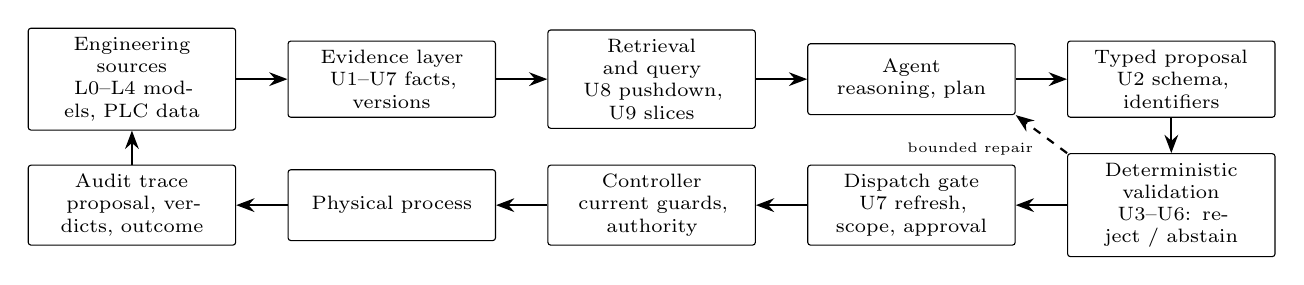
\begin{tikzpicture}[font=\scriptsize, box/.style={draw,rounded corners=1pt,align=center,minimum height=9mm,text width=24mm},arr/.style={-{Stealth},thick}]
\node[box] (src) at (0,0) {Engineering sources\\L0--L4 models, PLC data};
\node[box] (ev) at (3.3,0) {Evidence layer\\U1--U7 facts, versions};
\node[box] (q) at (6.6,0) {Retrieval and query\\U8 pushdown, U9 slices};
\node[box] (ag) at (9.9,0) {Agent\\reasoning, plan};
\node[box] (tp) at (13.2,0) {Typed proposal\\U2 schema, identifiers};
\node[box] (val) at (13.2,-1.6) {Deterministic validation\\U3--U6: reject / abstain};
\node[box] (gate) at (9.9,-1.6) {Dispatch gate\\U7 refresh, scope, approval};
\node[box] (plc) at (6.6,-1.6) {Controller\\current guards, authority};
\node[box] (proc) at (3.3,-1.6) {Physical process};
\node[box] (aud) at (0,-1.6) {Audit trace\\proposal, verdicts, outcome};
\draw[arr] (src)--(ev); \draw[arr] (ev)--(q); \draw[arr] (q)--(ag); \draw[arr] (ag)--(tp);
\draw[arr] (tp)--(val); \draw[arr] (val)--(gate); \draw[arr] (gate)--(plc); \draw[arr] (plc)--(proc);
\draw[arr] (proc)--(aud); \draw[arr] (aud)--(src);
\draw[arr,dashed] (val.north west) -- node[below left=-1pt,font=\tiny]{bounded repair} (ag.south east);
\end{tikzpicture}
\caption{Reference synthesis of runtime grounding. Evidence and validation support the agent;
dispatch and controller checks retain current-condition authority. No language model
participates in a hard-real-time loop.}
\label{fig:runtime}
\end{figure*}

Four properties follow from the analysis. (i) Validation distinguishes three dispositions:
reject when a violation is proved, abstain when required evidence is missing, and accept
only relative to the checked evidence contract. Absent evidence is not evidence of an
illegal command. (ii) A proposal accepted at planning time is revalidated at dispatch,
because state and observations change. (iii) Repair is bounded, names the violated rule,
and never weakens a guard or widens authorisation to avoid refusal. (iv) The semantic model
stays behind authenticated, parameterised query interfaces with versioned mappings rather
than being placed in the prompt or exposed as unrestricted graph or PLC access.

\section{Controlled Case Study}
\label{sec:case}

The case study asks whether capability gaps identified by AUF manifest as observable
grounding and validation failures. It uses an authored two-line bottling plant (17 assets,
73 signals, 22 shared descriptions, metric and imperial units, four interlocks, 14 feed
relations) with 35 tasks that declare their required facts and 137 proposed actions
(84 injected faults in 12 families, 53 legal). Context conditions C0--C4 expose
progressively more capabilities: tags and values; descriptions and unit symbols; a typed
\opcua{}/AAS-like profile; units, topology and taxonomy; and behaviour, guards and
provenance. Validator tiers G0--G4 check the same capability sets. Sufficiency is the
fraction of tasks whose declared facts are all present within a 6,000-token budget
(deterministic surrogate tokenizer); it is not a bound on model accuracy. Tasks, faults and
validators share one authored specification, so the study illustrates mechanisms and is
not an external validation.

\begin{table*}[t]
\centering\footnotesize
\setlength{\tabcolsep}{3pt}
\caption{CS1: progressive capability exposure on the authored reference plant (17 assets, 73 signals, 35 tasks, 84 faulty and 53 legal proposals). Suff.: declared required facts present at 6,000 surrogate tokens (not an accuracy bound). Context C$k$ is paired with validator G$k$.}
\label{tab:cs1}
\begin{tabular}{@{}llrrrlrr@{}}
\toprule
Ctx. & Projection & Top-1 & Verif. & Suff. & Val. & Recall & FPR \\
\midrule
C0 & OPC DA / PLC symbol table & 0\% & 0\% & 0\% & G0 & 0\% & 0\% \\
C1 & SCADA/historian CSV & 79\% & 0\% & 0\% & G1 & 14\% & 0\% \\
C2 & OPC UA NodeSet2 / AAS submodels & 95\% & 95\% & 23\% & G2 & 68\% & 8\% \\
C3 & RDF/OWL + QUDT + Brick + ISA-95 & 100\% & 100\% & 51\% & G3 & 74\% & 0\% \\
C4 & PackML + interlocks + SOSA/PROV & 100\% & 84\% & 86\% & G4 & 100\% & 0\% \\
\bottomrule
\end{tabular}
\end{table*}


\paragraph{CS1: Progressive exposure.} Top-1 grounding rises from \CsTopCOne{} with
descriptions to \CsTopCTwo{} with a typed profile, yet sufficiency at C2 is only
\CsSuffCTwo{}, rising to \CsSuffCFour{} at C4 (Table~\ref{tab:cs1}). Validator recall rises
from \CsRecallGTwo{} at G2, which also raises false alarms on \CsFPRGTwo{} of legal actions
through literal unit comparison, to \CsRecallGFour{} at G4 without false alarms. Typing
resolves the target but not whether the action is admissible.

\begin{table}[t]
\centering\footnotesize
\setlength{\tabcolsep}{3pt}
\caption{CS2: retrieval strategy crossed with exposed capabilities at 6,000 surrogate tokens. Membership and graph retrieval share a fixed entity resolver; graph traversal requires C3/C4 relations.}
\label{tab:cs2}
\begin{tabular}{@{}llrrr@{}}
\toprule
Ctx. & Retrieval & Suff. & Coverage & Tokens \\
\midrule
C2 & lexical & 23\% & 55\% & 5193 \\
C2 & membership & 23\% & 48\% & 1906 \\
C3 & lexical & 40\% & 67\% & 5075 \\
C3 & membership & 29\% & 59\% & 2507 \\
C3 & graph & 46\% & 76\% & 5341 \\
C4 & lexical & 71\% & 85\% & 5107 \\
C4 & membership & 46\% & 69\% & 2767 \\
C4 & graph & 80\% & 93\% & 5345 \\
\bottomrule
\end{tabular}
\end{table}

\begin{table}[t]
\centering\footnotesize
\setlength{\tabcolsep}{3pt}
\caption{CS3: removing one AUF capability at a time from the full C4/G4 configuration. Abstentions on missing evidence are not counted as detections.}
\label{tab:cs3}
\begin{tabular}{@{}lrrr@{}}
\toprule
Removed & Suff. & Recall & Abstain \\
\midrule
none & 80\% & 100\% & 0 \\
behaviour & 63\% & 89\% & 37 \\
constraints & 69\% & 96\% & 20 \\
provenance & 74\% & 85\% & 40 \\
topology & 63\% & 94\% & 5 \\
units & 80\% & 61\% & 60 \\
\bottomrule
\end{tabular}
\end{table}


\paragraph{CS2: Retrieval.} At equal budget, graph traversal yields the highest
sufficiency where relations exist, membership-scoped retrieval is cheapest but omits
evidence, and lexical retrieval cannot compensate for capabilities the context lacks
(Table~\ref{tab:cs2}). Evidence availability and retrieval are separate variables.

\paragraph{CS3: Capability removal.} Removing one capability at a time reduces sufficiency,
recall or both, and turns detections into abstentions on missing evidence
(Table~\ref{tab:cs3}). Removing unit semantics leaves task sufficiency unchanged in this
budget yet causes the largest loss of fault recall: the effect of a capability depends on
whether it is needed to answer or to check.

\begin{table}[t]
\centering\footnotesize
\setlength{\tabcolsep}{3pt}
\caption{CS4: equally informed procedural and SHACL validators on identical engineering facts.}
\label{tab:cs4}
\begin{tabular}{@{}lrrr@{}}
\toprule
Validator & Faults caught & False alarms & Diagnosis \\
\midrule
Procedural & 84/84 & 0/53 & 100\% \\
SHACL & 84/84 & 0/53 & 100\% \\
\bottomrule
\end{tabular}
\end{table}


\paragraph{CS4: Representation versus information.} A procedural validator and a SHACL
validator given identical engineering facts produce \CsDisagreements{} raw-family
disagreements (Table~\ref{tab:cs4}). The measured benefit lies in explicit engineering
evidence, not in the validation technology; reuse, auditability and maintenance effort
remain to be measured.

\begin{table}[t]
\centering\footnotesize
\setlength{\tabcolsep}{3pt}
\caption{CS5: matched facts recovered from the emitted OPC UA NodeSet2 and AAS v3 projections of the same plant ($\neq$: conflicting value). Both projections are generated from one specification, so this measures the emitted profiles, not limits of either standard.}
\label{tab:cs5}
\begin{tabular}{@{}llrrr@{}}
\toprule
Fact & AUF & OPC UA & AAS & Union \\
\midrule
identity & U1 & 73/73 & 73/73 & 73/73 \\
semantic id & U1 & 0/46 & 46/46 & 46/46 \\
nameplate & U1 & 0/11 & 11/11 & 11/11 \\
datatype & U2 & 73/73 & 73/73 & 73/73 \\
access & U2 & 73/73 & 0/73 & 73/73 \\
range & U2 & 73/73 & 0/73 & 73/73 \\
unit & U3 & 73/73 & 73/73 & 73/73 \\
quantity kind & U3 & 53/73 (20$\neq$) & 0/73 & 53/73 (20$\neq$) \\
membership & U4 & 73/73 & 73/73 & 73/73 \\
parent & U4 & 16/16 & 0/16 & 16/16 \\
feeds & U4 & 0/14 & 0/14 & 0/14 \\
state & U5 & 0/9 & 9/9 & 9/9 \\
legal commands & U5 & 0/9 & 0/9 & 0/9 \\
interlock & U6 & 0/4 & 0/4 & 0/4 \\
value & U7 & 0/53 & 53/53 & 53/53 \\
observation time & U7 & 0/53 & 0/53 & 0/53 \\
\bottomrule
\end{tabular}
\end{table}


\paragraph{CS5: OPC~UA versus AAS.} The plant's \opcua{} NodeSet2 and AAS v3 projections
were parsed back into \CsFacts{} matched facts (Table~\ref{tab:cs5}). The \opcua{} profile
recovers \CsOpcuaFacts{} (\CsOpcuaPct{}), including access levels, engineering ranges and
hierarchy; the AAS profile recovers \CsAasFacts{} (\CsAasPct{}), including semantic
identifiers, nameplates, operating state and values; their union reaches \CsUnionFacts{}
(\CsUnionPct{}). \opcua{} \texttt{EUInformation} is attached to the unit, so
\CsQkConflicts{} count-type signals report the unit's quantity kind rather than the
signal's. Neither projection carries flow topology, legal commands, interlocks or
observation timestamps, which C4 requires. The serialisations cost \CsOpcuaTokens{} and
\CsAasTokens{} surrogate tokens. Both standards can express more through companion models,
qualifiers or additional submodels; the result shows that the emitted profiles are
complementary and jointly incomplete, not that either standard is inferior. A second,
derived pilot, an IIH-attributed KUKA robot NodeSet and its loss-aware AAS projection,
retains all \CsKukaRetained{} of \CsKukaFacts{} source facts, including 90 nodes and
277 references; it verifies conversion fidelity only.

\section{Open Challenges and Research Agenda}
\label{sec:challenges}

\paragraph{Semantic completeness.} Validation is only as complete as the modelled guards.
Methods are needed to show that an interlock inventory matches the control logic, for
example by extracting guards from PLC programs and cross-checking them with declared
constraints.

\paragraph{Semantic correctness.} A graph can conform to every shape and still be wrong.
Unit consistency with process equations, declared topology versus P\&IDs, and the
equivalence of constraint models and ladder logic are decidable checks that are not yet
routine. An incorrect semantic layer is more dangerous than none because it is trusted.

\paragraph{Runtime freshness and dispatch races.} Engineering semantics combined with stale
observations remain unsafe. Agents need freshness contracts, revalidation at dispatch and
measured behaviour under reconnects, subscription lag and state changes between planning
and execution.

\paragraph{Agent and controller authority.} The boundary between supervisory reasoning and
deterministic control needs explicit design: which checks the gateway performs, which remain
in the controller, and how rejections and acknowledgements are traced.

\paragraph{Model evolution and transfer.} PLC programs, configurations and mappings change.
How semantic constraints are versioned, migrated and transferred between machines, and at
what engineering cost, is largely unmeasured; reuse and maintainability claims for
declarative constraints require change-effort studies.

\paragraph{Engineering cost and ownership.} Someone must author and maintain identity maps,
unit bindings, state models and guards. Bootstrapping from existing artefacts (\opcua{}
address spaces, AutomationML, DEXPI, PLC projects) with formal acceptance checks is a
promising route.

\paragraph{Benchmarks with actions and consequences.} Industrial grounding lacks shared
benchmarks with real installations, independently authored tasks, labelled faulty and
legal actions, severity-weighted scoring and physical outcomes; the synthetic corpus used
here is a starting point, not a substitute.

\paragraph{Safety assurance.} Semantic validation is not functional safety. Zero observed
invalid actions in a test corpus establishes no safety integrity level; assurance cases
must separate proposal quality, gateway rejection and controller protection.

\paragraph{Authorisation and policy.} Agents need the analogue of operator competence and
shift authorisation, joining policy languages and security frameworks
\cite{w3c2018odrl,iec62443} to equipment models and plant states.

\paragraph{Agent-ready standards.} Existing standards were designed for interoperability.
Publishing constraints and legal-command models alongside information models, for instance
as a versioned constraint submodel or companion specification, would close the largest gap
identified by the capability analysis.

\section{Threats to Validity and Conclusion}
\label{sec:conclusion}

\paragraph{Threats to validity.} The search may miss grey literature and vendor work, and
arXiv records are not peer reviewed; snowballing and labelling mitigate but do not remove
this. AUF scores are first-rater codes based on default specifications until the second
rater's agreement is reported, and optional extensions or deployed profiles can change
judgements. The capability list was derived top-down and is tested for saturation against
the coded corpus. The case study uses one authored plant whose tasks, faults and
validators share a specification; its OPC~UA/AAS comparison measures emitted profiles from
that specification. No physical trial or complete model evaluation is reported; the
surrogate tokenizer does not measure billing tokens.

\paragraph{Conclusion.} Industrial AI-agent reliability depends less on the choice of
language model or semantic syntax than on whether the agent has access to explicit,
current, machine-interpretable engineering evidence covering identity, quantities,
relations, behaviour, constraints and provenance. Existing standards provide many of
these capabilities, but they are fragmented across technologies and rarely exposed as a
coherent runtime evidence contract. The case study shows the consequences: typing alone
resolves targets but not admissibility, equally informed validators decide identically,
and matched \opcua{} and AAS profiles are complementary yet jointly incomplete. Making
industrial standards agent-ready, chiefly by publishing behaviour and constraints with
provenance behind query interfaces, is the most consequential next step.


\bibliographystyle{IEEEtran}
\bibliography{refs}

\end{document}
